\section{Results} \label{sec:Results}

%%%%%%%%%%%%%%%%%%%%%%%%%%%%%%%%%%%%%%%%%%%%%%%%%%%%%%%%%%%%%%%%%%%%%%%%%%%  
%% JUST THE OBJECTIVE FACTS, no interpretation or discussion
%%
%% what exactly did you do
%%  
%% what were the inputs/outputs/parameters
%%  
%% what computer hardware
%%  
%% what software
%%  
%% what were the results
%%  
%% tables/figures/plots
%%  
%% error analysis
%%%%%%%%%%%%%%%%%%%%%%%%%%%%%%%%%%%%%%%%%%%%%%%%%%%%%%%%%%%%%%%%%%%%%%%%%%%  

Here we shall present the results we acquired from our experiments. We will
describe our generic testbed, so should the reader wish to follow along in
real time they may have the option of doing so. After this, the performance 
of each brain will be evaluated individually.

\subsection{Testbed}
All of our experiments were performed within the Flatworld II v.1.0 
environment. Our code was writen in Python 2.6, and interfaced with 
Flatworld's C-based API via a shim (see section \ref{sec:Ack}). All of our
runs were done on a Lenovo Ideapad T430 with an Intel i7 quad core processor
and 16GB of DDR3 RAM. Windows 7 Pro 64bit is the machine's native platform,
but we ran our tests inside a virtual machine using VMware 8.04. The virtual
machine was configured with Ubuntu 10.04 32bit, 1GB of RAM and a single 2GHz
processor.


\subsection{Brain 0}
We start our data presentation with Brain 0 (a very good place to start).
It should come as no surprise that brain 0's lifespan is 2000 time steps. 
The agent makes no moves, and makes no attempts to eat anything. 
Figure \ref{fig:brain0energy} shows an agent's average energy depletion over 
time based upon 153 runs. The bar has been set, as they say.

\begin{figure}
\begin{center}
  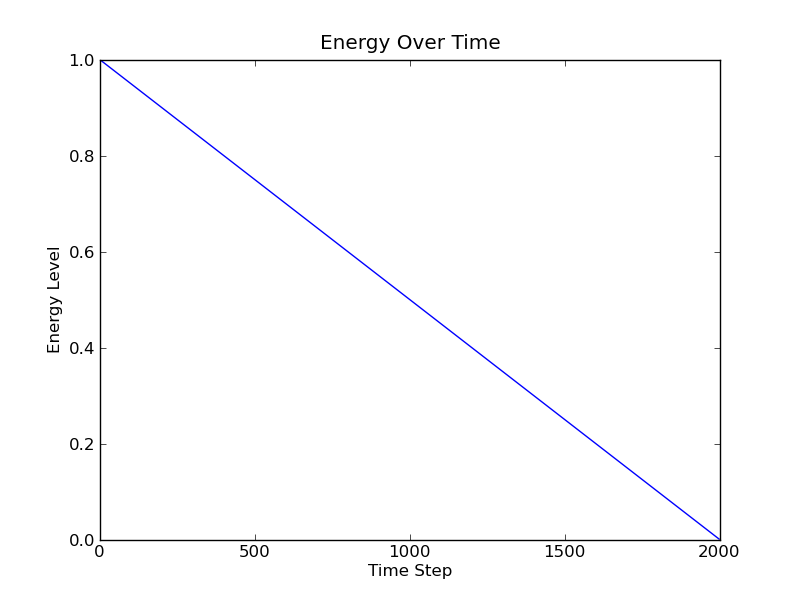
\includegraphics[scale=.65]{plots/brain0energy.png}
  \caption{Agent's energy level over time ($\sigma = 0$)}
  \label{fig:brain0energy}
\end{center}
\end{figure}

Figure \ref{fig:brain0his} is a histogram which also confirms the average 
lifespan of our agents to be exactly 2000 time steps.

\begin{figure}
\begin{center}
  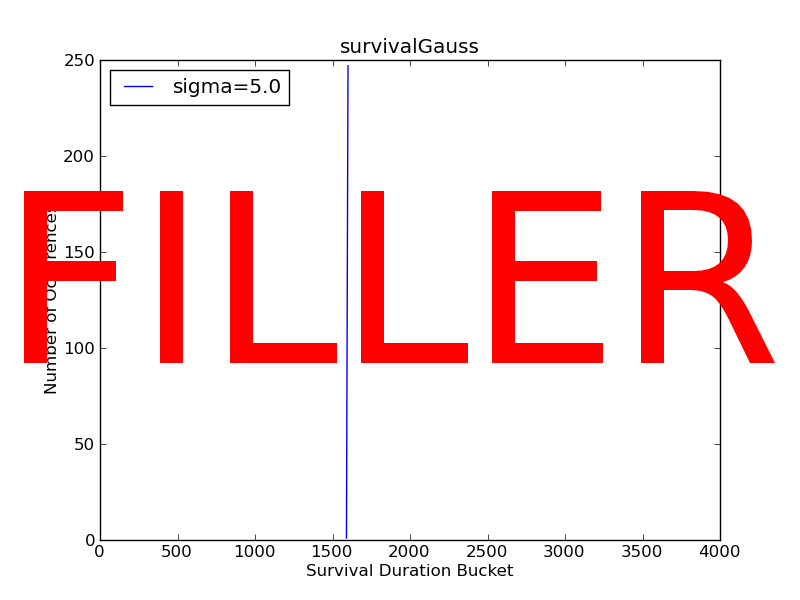
\includegraphics[scale=.65]{plots/filler.png}
  \caption{Agent lifetimes for Brain 0 ($\sigma = 0$)}
  \label{fig:brain0his}
\end{center}
\end{figure}


\subsection{Brain 1}
It should come as no surprise that Brain 1's performance will show
little improvement upon Brain 0. This is due to the fact that not only is
it relying on food to be directly in its path, but it also is expending 
\emph{more} energy from the act of moving. Figure \ref{fig:brain1velo} shows
that increasing the agent's velocity will cause its energy to decrease
exponentially.

\begin{figure}
\begin{center}
  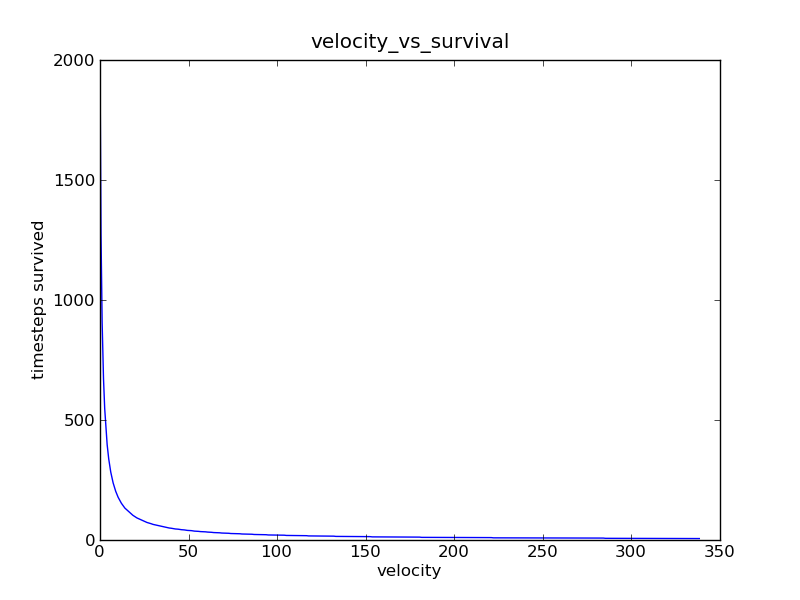
\includegraphics[scale=.65]{plots/brain1velo.png}
  \caption{An agent's lifespan as a function of velocity}
  \label{fig:brain1velo}
\end{center}
\end{figure}

\begin{figure}
\begin{center}
  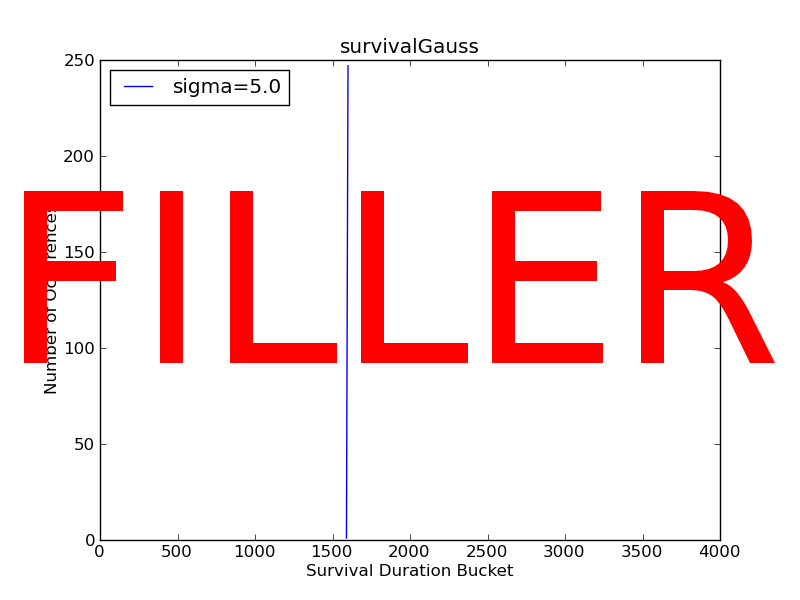
\includegraphics[scale=.65]{plots/filler.png}
  \caption{Agent lifetimes for Brain 1 {\Large NEA GET SIGMA}($\sigma = 0$)}
  \label{fig:brain1his}
\end{center}
\end{figure}

In these fledgling stages, velocity is indeed critical to longevity. The
histogram in figure \ref{fig:brain1his} illustrates agents' lifetimes based
off of a constant velocity value of {\Large VELOCITY VALUE IS WHAT?}
